\section{Experimental Evaluation and Results}
\label{sec:experiments}

\subsection{Protocol}

Each run generates a seeded synthetic city of $N = 16$ units over $T = 18$
steps, applies one of the four policy scenarios, and forms rolling history
windows of length $W_h = 4$ with next-step targets. The split is strictly
temporal---the earliest $70\%$ of windows train, the remainder test---with no
shuffling, so no future information reaches the training set. The scaler of
Section~\ref{subsec:scaling} is fit on the training windows alone.

We restrict the modelled feature set to the three spillover-bearing channels
(land value, rent, accessibility). All four models are constructed under an
identical random seed immediately before instantiation, so that comparisons
between architectures, and between topology conditions, reflect the quantity
under study rather than the draw of the initial weights. Learned models train
for $250$ epochs with Adam at learning rate $10^{-3}$ under a mean squared
error objective; persistence is parameter-free and is never trained. Metrics
are computed after inverting the scaler, pooled over every window, unit and
feature, so the reported RMSE is a true root-mean-squared error rather than a
root-mean-square of per-window absolute errors.

The full design is $10$ seeds $\times$ $4$ scenarios $\times$ $4$ models for
the main sweep, plus $10$ seeds $\times$ $4$ scenarios $\times$ $2$ ablated
topologies for \CGCEN{}, giving $240$ fitted models. Aggregate statistics use
the sample standard deviation ($\mathrm{ddof} = 1$) and Student-$t$ $95\%$
confidence intervals. Model comparisons use two-sided paired $t$-tests over
seeds, pairing on the seed so that between-seed variance in task difficulty is
differenced out.

\subsection{Forecast Accuracy}

Table~\ref{tab:benchmark_results} reports per-scenario MAE and RMSE with
significance markers; Figure~\ref{fig:model-comparison} summarises the pooled
comparison.

\begin{table*}[t]
\centering
\caption{Forecast accuracy across policy scenarios on the synthetic CivicTwin panel. Values are mean $\pm$ standard deviation of the pooled test-set error over independent seeds. Significance markers denote a paired $t$-test of each baseline against the Causal ST-GNN on MAE ($^{*}p<0.05$, $^{**}p<0.01$, $^{***}p<0.001$).}
\label{tab:benchmark_results}
\small
\begin{tabular}{lcccccccc}
\toprule
\textbf{Model} & \multicolumn{2}{c}{\textbf{Baseline}} & \multicolumn{2}{c}{\textbf{Market-Led Development}} & \multicolumn{2}{c}{\textbf{Inclusionary Housing}} & \multicolumn{2}{c}{\textbf{Land-Value Capture}} \\
\cmidrule(lr){2-3}\cmidrule(lr){4-5}\cmidrule(lr){6-7}\cmidrule(lr){8-9}
 & MAE & RMSE & MAE & RMSE & MAE & RMSE & MAE & RMSE \\
\midrule
Causal ST-GNN (CG-CEN) & $9.901 \pm 2.234$ & $15.482 \pm 2.994$ & $8.671 \pm 2.954$ & $13.763 \pm 4.719$ & $8.645 \pm 2.368$ & $13.316 \pm 3.630$ & $8.303 \pm 1.991$ & $12.688 \pm 2.981$ \\
Spatial Lag Model & $11.837 \pm 3.234$ & $19.269 \pm 5.083$ & $12.014 \pm 3.283^{**}$ & $19.595 \pm 5.167$ & $11.796 \pm 3.231^{**}$ & $19.135 \pm 5.075$ & $11.834 \pm 3.240^{**}$ & $19.181 \pm 5.096$ \\
Temporal MLP & $20.154 \pm 8.574^{**}$ & $34.996 \pm 15.895$ & $21.119 \pm 8.560^{**}$ & $36.780 \pm 15.935$ & $19.450 \pm 7.934^{**}$ & $33.244 \pm 14.950$ & $19.404 \pm 7.944^{***}$ & $33.138 \pm 14.987$ \\
Naive Persistence & $27.870 \pm 1.299^{***}$ & $37.487 \pm 1.921$ & $28.266 \pm 1.319^{***}$ & $38.202 \pm 1.976$ & $27.697 \pm 1.287^{***}$ & $37.173 \pm 1.881$ & $27.774 \pm 1.289^{***}$ & $37.306 \pm 1.882$ \\
\midrule
\textit{p} vs. ST-GNN (MAE) & \multicolumn{2}{c}{$<0.001$} & \multicolumn{2}{c}{$<0.001$} & \multicolumn{2}{c}{$<0.001$} & \multicolumn{2}{c}{$<0.001$} \\
\bottomrule
\end{tabular}
\end{table*}


Pooled across all four scenarios on the real topology, \CGCEN{} attains
$\mathrm{MAE} = 8.88 \pm 2.40$, against $11.87 \pm 3.12$ for the Spatial Lag
Model, $20.03 \pm 7.97$ for the Temporal MLP, and $27.90 \pm 1.27$ for Naive
Persistence. The RMSE ordering is identical ($13.81$, $19.30$, $34.54$,
$37.54$), indicating that \CGCEN{}'s advantage is not an artefact of a few
well-predicted units but holds under a loss that penalises large residuals more
heavily.

The margin over the graph-blind MLP is substantial and significant in every
scenario, with mean differences between $-10.25$ and $-12.45$ MAE and
$p$-values from $9.4 \times 10^{-4}$ to $5.8 \times 10^{-3}$. The margin over
persistence is larger still ($p < 2 \times 10^{-8}$ throughout). We regard the
persistence comparison as a sanity floor rather than a result: in an earlier
iteration of this work both learned baselines lost to it, which is what first
revealed that the benchmark was mis-specified.

\subsection{Where the Graph Earns Its Keep}

The comparison against the Spatial Lag Model is the substantive one, because
the SLM is itself graph-aware and differs from \CGCEN{} principally in
functional form. Here the result is conditional, and we report the condition
rather than the pooled average:

\begin{center}
\begin{tabular}{lrrr}
\toprule
\textbf{Scenario} & $\Delta$\textbf{MAE} & $t$ & $p$ \\
\midrule
Baseline              & $-1.94$ & $-1.68$ & $0.127$ \\
Market-Led            & $-3.34$ & $-4.14$ & $0.0025$ \\
Inclusionary Housing  & $-3.15$ & $-3.96$ & $0.0033$ \\
Land-Value Capture    & $-3.53$ & $-4.50$ & $0.0015$ \\
\bottomrule
\end{tabular}
\end{center}

\CGCEN{} beats the SLM by roughly $3.3$ MAE under every active intervention,
with large paired effect sizes (Cohen's $d_z$ between $-1.25$ and $-1.42$), but
its $1.94$ MAE advantage in the untreated baseline does not reach significance
at $n = 10$ seeds ($p = 0.127$, $d_z = -0.53$).

This boundary is, we believe, the most useful result in the paper. In a static
equilibrium the system's spatial structure is adequately summarised by a linear
autoregressive lag, and the additional capacity of a nonlinear message-passing
model buys nothing that survives seed variance. It is only when policy
interventions inject treatment-dependent, spatially propagating perturbations
that the nonlinear interference channel $\Psi$ has structure to exploit. A
paper reporting only the pooled comparison would have claimed a general
forecasting advantage that the per-scenario decomposition does not support.

\subsection{Topology Ablation}

To establish that \CGCEN{}'s advantage derives from the graph rather than from
architectural capacity, we re-fit it under two counterfactual topologies while
holding everything else fixed: \emph{no edges}, in which the interference term
of \eqref{eq:decomposition} is identically zero, and \emph{shuffled}, in which
the edge index is remapped through a random node permutation, preserving the
degree sequence and edge count while destroying the correspondence between
graph structure and spatial reality.

\begin{center}
\begin{tabular}{lrrl}
\toprule
\textbf{Topology} & \textbf{MAE} & \textbf{Degradation} & \textbf{$p$ vs.\ real} \\
\midrule
Real graph      & $8.88$  & ---     & --- \\
No edges        & $11.77$ & $+2.89$ & $0.005$--$0.008$ (3/4) \\
Shuffled edges  & $13.76$ & $+4.88$ & $0.0001$--$0.018$ (4/4) \\
\bottomrule
\end{tabular}
\end{center}

Removing the graph costs $2.89$ MAE, a $32.6\%$ relative degradation.
Randomising it costs $4.88$ MAE, a $55.0\%$ degradation, significant in all
four scenarios.

The critical observation is that \emph{shuffled is worse than no edges}. If the
model were merely using message passing as a generic smoothing or
regularisation device, a random graph would serve about as well as the true
one, and both would sit between the real graph and the edgeless condition.
Instead, supplying a structurally plausible but factually wrong topology is
more damaging than supplying none at all. This is the signature of a model that
has learned the specific adjacency: it propagates neighbour information with
confidence, and when that information is drawn from the wrong neighbours the
confident propagation actively injects error.
Figure~\ref{fig:ablation} shows the per-scenario breakdown.

For contrast, the same ablation under the static-shock generator of
Section~\ref{subsec:collapse} gave no-edges $14.16$ against real $14.82$---the
edgeless model was \emph{better}---and shuffled indistinguishable from real
($p = 0.70$--$0.93$). The ablation is thus not merely a confirmation of the
final model; it is the diagnostic that distinguished a working benchmark from a
degenerate one.

\subsection{Causal Channel Behaviour}

Figure~\ref{fig:spillover} visualises the estimated direct and interference
effects on the lattice. The ITE surface concentrates on the treated boundary,
as it must: by \eqref{eq:ite}, $\tau_i$ is identically zero at untreated units.
The STE surface spreads outward from the treated set with magnitude decaying in
graph distance, and is exactly zero at units with no treated neighbour. These
are structural guarantees of the decomposition rather than learned behaviour,
and we verify both as unit tests together with the additive identity
$\hat{Y} = \Phi + \sum_j W_{ij}\Psi$.

\subsection{Policy Scorecard}

Table~\ref{tab:policy_scorecard} ranks the scenarios by displacement-pressure
mitigation. With the level-aware term of \eqref{eq:dpi} active, the contrasts
are substantively legible: Market-Led Development raises $\DPI$ by
$+0.0172 \pm 0.0007$ relative to baseline, while Inclusionary Housing and
Land-Value Capture lower it by $-0.0131 \pm 0.0006$ and $-0.0125 \pm 0.0005$
respectively. The two mitigating policies are close but consistently ordered
across seeds, with inclusionary housing marginally ahead---unsurprising, since
it acts on both rent and housing stock while land-value capture acts on rent
alone.

Under the growth-rate-only specification these same contrasts were on the order
of $10^{-4}$ and returned to zero within one step of the intervention. The
level-aware term increases the measured effect by more than two orders of
magnitude and, as panel (d) of Figure~\ref{fig:trajectories} shows, sustains it
across the full horizon. We stress that this is a change in what the index
\emph{measures}, not a change in the underlying simulated economy: the panels
are identical, and only the readout differs.

\begin{table}[t]
\centering
\caption{Policy scenario scorecard ranked by displacement-pressure mitigation. Negative values indicate that the intervention reduces the index relative to the untreated baseline panel. Values are means over independent seeds.}
\label{tab:policy_scorecard}
\small
\begin{tabular}{clccc}
\toprule
\textbf{Rank} & \textbf{Scenario} & $\Delta$\textbf{DPI} & $\Delta$\textbf{H+T} & $\Delta$\textbf{Rent/Income} \\
\midrule
1 & Inclusionary Housing & $-0.01305 \pm 0.00055$ & $-0.00005 \pm 0.00000$ & $-4.668e-05$ \\
2 & Land-Value Capture & $-0.01255 \pm 0.00054$ & $-0.00004 \pm 0.00000$ & $-4.481e-05$ \\
3 & Baseline & $0.00000 \pm 0.00000$ & $0.00000 \pm 0.00000$ & $0.000e+00$ \\
4 & Market-Led Development & $0.01721 \pm 0.00073$ & $0.00006 \pm 0.00000$ & $6.145e-05$ \\
\bottomrule
\end{tabular}
\end{table}


\begin{figure*}[t]
  \centering
  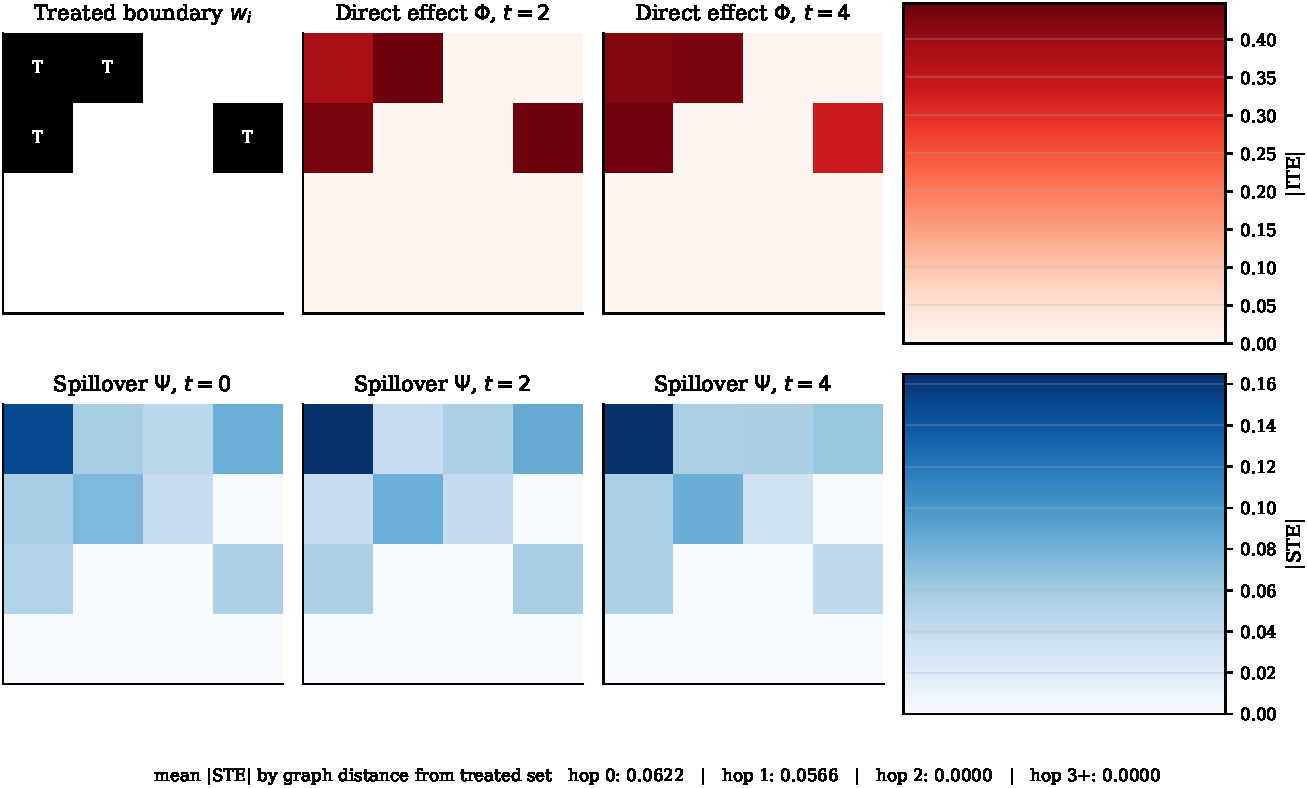
\includegraphics[width=\textwidth]{spillover_heatmaps.pdf}
  \caption{Direct policy impact versus multi-hop neighbour spillover on the
  $4 \times 4$ lattice under the Market-Led scenario. Top row: treated boundary
  and the $|\ITE|$ surface from $\Phi$. Bottom row: the $|\STE|$ surface from
  the neighbour-aggregated $\Psi$ at three evaluation steps. The ITE is exactly
  zero at untreated units and the STE is exactly zero at units with no treated
  neighbour, both by construction of \eqref{eq:ite}--\eqref{eq:ste}.}
  \label{fig:spillover}
\end{figure*}

\begin{figure*}[t]
  \centering
  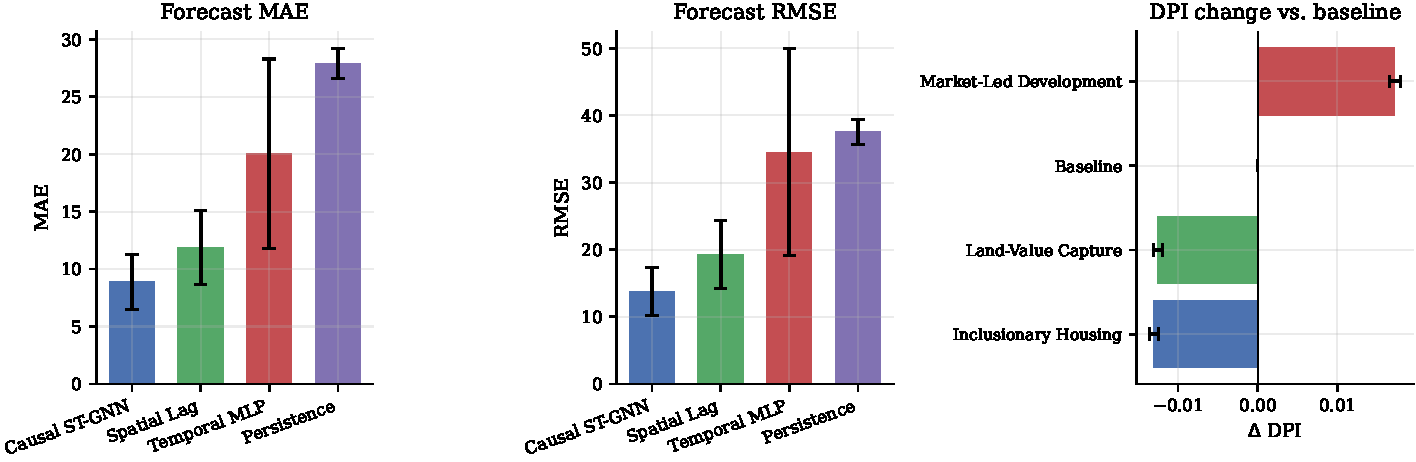
\includegraphics[width=\textwidth]{model_comparison_bar.pdf}
  \caption{Model family comparison pooled over ten seeds and four scenarios
  (left, centre) and policy $\DPI$ mitigation relative to the untreated
  baseline (right). Error bars are one standard deviation across seeds.}
  \label{fig:model-comparison}
\end{figure*}

\begin{figure*}[t]
  \centering
  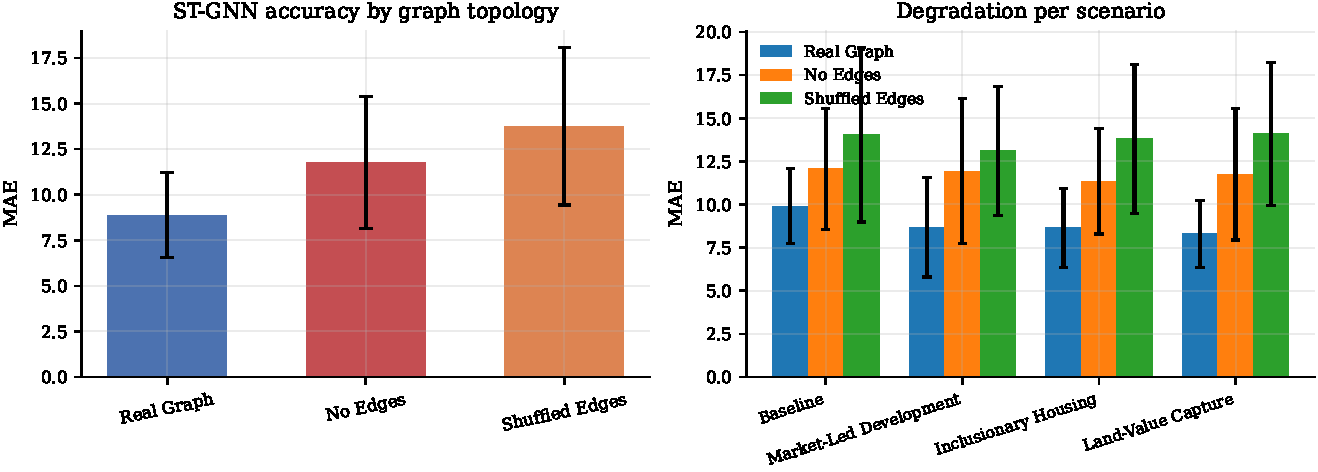
\includegraphics[width=\textwidth]{ablation_topology.pdf}
  \caption{Graph topology ablation. Left: pooled \CGCEN{} accuracy under the
  real graph, an edgeless graph and a randomly rewired graph of identical
  degree sequence. Right: per-scenario breakdown. Randomising the topology is
  more damaging than removing it, indicating the model has learned the specific
  adjacency rather than using message passing as generic smoothing.}
  \label{fig:ablation}
\end{figure*}
